\PassOptionsToPackage{unicode=true}{hyperref} % options for packages loaded elsewhere
\PassOptionsToPackage{hyphens}{url}
%
\documentclass[10pt,xcolor=table,color={dvipsnames,usenames},ignorenonframetext,usepdftitle=false,french]{beamer}
\setbeamertemplate{caption}[numbered]
\setbeamertemplate{caption label separator}{: }
\setbeamercolor{caption name}{fg=normal text.fg}
\beamertemplatenavigationsymbolsempty
\usepackage{caption}
\captionsetup{skip=0pt,belowskip=0pt}
%\setlength\abovecaptionskip{-15pt}
\usepackage{lmodern}
\usepackage{amssymb,amsmath,mathtools,multirow}
\usepackage{float,hhline}
\usepackage{tikz}
\usepackage[tikz]{bclogo}
\usepackage{mathtools}
\usepackage{ifxetex,ifluatex}
\usepackage{fixltx2e} % provides \textsubscript
\ifnum 0\ifxetex 1\fi\ifluatex 1\fi=0 % if pdftex
  \usepackage[T1]{fontenc}
  \usepackage[utf8]{inputenc}
  \usepackage{textcomp} % provides euro and other symbols
\else % if luatex or xelatex
  \usepackage{unicode-math}
  \defaultfontfeatures{Ligatures=TeX,Scale=MatchLowercase}
\fi
\usetheme[coding=utf8,language=english,
,titlepagelogo=img/SACElogo.jpg
]{TorinoTh}
% use upquote if available, for straight quotes in verbatim environments
\IfFileExists{upquote.sty}{\usepackage{upquote}}{}
% use microtype if available
\IfFileExists{microtype.sty}{%
\usepackage[]{microtype}
\UseMicrotypeSet[protrusion]{basicmath} % disable protrusion for tt fonts
}{}
\IfFileExists{parskip.sty}{%
\usepackage{parskip}
}{% else
\setlength{\parindent}{0pt}
\setlength{\parskip}{6pt plus 2pt minus 1pt}
}
\usepackage{hyperref}
\hypersetup{
            pdftitle={RJDemetra: an R interface to JDemetra+},
            pdfauthor={Alain Quartier-la-Tente},
            pdfborder={0 0 0},
            breaklinks=true}
\urlstyle{same}  % don't use monospace font for urls
\newif\ifbibliography
\usepackage{color}
\usepackage{fancyvrb}
\newcommand{\VerbBar}{|}
\newcommand{\VERB}{\Verb[commandchars=\\\{\}]}
\DefineVerbatimEnvironment{Highlighting}{Verbatim}{commandchars=\\\{\}}
% Add ',fontsize=\small' for more characters per line
\usepackage{framed}
\definecolor{shadecolor}{RGB}{248,248,248}
\newenvironment{Shaded}{\begin{snugshade}}{\end{snugshade}}
\newcommand{\AlertTok}[1]{\textcolor[rgb]{0.94,0.16,0.16}{#1}}
\newcommand{\AnnotationTok}[1]{\textcolor[rgb]{0.56,0.35,0.01}{\textbf{\textit{#1}}}}
\newcommand{\AttributeTok}[1]{\textcolor[rgb]{0.77,0.63,0.00}{#1}}
\newcommand{\BaseNTok}[1]{\textcolor[rgb]{0.00,0.00,0.81}{#1}}
\newcommand{\BuiltInTok}[1]{#1}
\newcommand{\CharTok}[1]{\textcolor[rgb]{0.31,0.60,0.02}{#1}}
\newcommand{\CommentTok}[1]{\textcolor[rgb]{0.56,0.35,0.01}{\textit{#1}}}
\newcommand{\CommentVarTok}[1]{\textcolor[rgb]{0.56,0.35,0.01}{\textbf{\textit{#1}}}}
\newcommand{\ConstantTok}[1]{\textcolor[rgb]{0.00,0.00,0.00}{#1}}
\newcommand{\ControlFlowTok}[1]{\textcolor[rgb]{0.13,0.29,0.53}{\textbf{#1}}}
\newcommand{\DataTypeTok}[1]{\textcolor[rgb]{0.13,0.29,0.53}{#1}}
\newcommand{\DecValTok}[1]{\textcolor[rgb]{0.00,0.00,0.81}{#1}}
\newcommand{\DocumentationTok}[1]{\textcolor[rgb]{0.56,0.35,0.01}{\textbf{\textit{#1}}}}
\newcommand{\ErrorTok}[1]{\textcolor[rgb]{0.64,0.00,0.00}{\textbf{#1}}}
\newcommand{\ExtensionTok}[1]{#1}
\newcommand{\FloatTok}[1]{\textcolor[rgb]{0.00,0.00,0.81}{#1}}
\newcommand{\FunctionTok}[1]{\textcolor[rgb]{0.00,0.00,0.00}{#1}}
\newcommand{\ImportTok}[1]{#1}
\newcommand{\InformationTok}[1]{\textcolor[rgb]{0.56,0.35,0.01}{\textbf{\textit{#1}}}}
\newcommand{\KeywordTok}[1]{\textcolor[rgb]{0.13,0.29,0.53}{\textbf{#1}}}
\newcommand{\NormalTok}[1]{#1}
\newcommand{\OperatorTok}[1]{\textcolor[rgb]{0.81,0.36,0.00}{\textbf{#1}}}
\newcommand{\OtherTok}[1]{\textcolor[rgb]{0.56,0.35,0.01}{#1}}
\newcommand{\PreprocessorTok}[1]{\textcolor[rgb]{0.56,0.35,0.01}{\textit{#1}}}
\newcommand{\RegionMarkerTok}[1]{#1}
\newcommand{\SpecialCharTok}[1]{\textcolor[rgb]{0.00,0.00,0.00}{#1}}
\newcommand{\SpecialStringTok}[1]{\textcolor[rgb]{0.31,0.60,0.02}{#1}}
\newcommand{\StringTok}[1]{\textcolor[rgb]{0.31,0.60,0.02}{#1}}
\newcommand{\VariableTok}[1]{\textcolor[rgb]{0.00,0.00,0.00}{#1}}
\newcommand{\VerbatimStringTok}[1]{\textcolor[rgb]{0.31,0.60,0.02}{#1}}
\newcommand{\WarningTok}[1]{\textcolor[rgb]{0.56,0.35,0.01}{\textbf{\textit{#1}}}}
\usepackage{graphicx,grffile}
\makeatletter
\def\maxwidth{\ifdim\Gin@nat@width>\linewidth\linewidth\else\Gin@nat@width\fi}
\def\maxheight{\ifdim\Gin@nat@height>\textheight\textheight\else\Gin@nat@height\fi}
\makeatother
% Scale images if necessary, so that they will not overflow the page
% margins by default, and it is still possible to overwrite the defaults
% using explicit options in \includegraphics[width, height, ...]{}
\setkeys{Gin}{width=\maxwidth,height=\maxheight,keepaspectratio}
% Prevent slide breaks in the middle of a paragraph:
\widowpenalties 1 10000
\raggedbottom
\AtBeginPart{
  \let\insertpartnumber\relax
  \let\partname\relax
  \frame{\partpage}
}
\AtBeginSection{
  \ifbibliography
  \else
    \begin{frame}{Sommaire}
    \tableofcontents[currentsection, hideothersubsections]
    \end{frame}
  \fi
}
\setlength{\emergencystretch}{3em}  % prevent overfull lines
\providecommand{\tightlist}{%
  %\setlength{\itemsep}{0pt}
  \setlength{\parskip}{0pt}
  }
\setcounter{secnumdepth}{0}

% set default figure placement to htbp
\makeatletter
\def\fps@figure{htbp}
\makeatother

\usepackage{wrapfig}
\usepackage{booktabs}
\usepackage{longtable}
\usepackage{array}
\usepackage{multirow}
\usepackage[table]{xcolor}
\usepackage{wrapfig}
\usepackage{float}
\usepackage{colortbl}
\usepackage{pdflscape}
\usepackage{tabu}
\usepackage{threeparttable}
\usepackage{threeparttablex}
\usepackage[normalem]{ulem}
\usepackage{makecell}
\usepackage{animate}
\usepackage{fontawesome5}

\title{RJDemetra: an R interface to JDemetra+}
\ateneo{useR!2019}
\author{Alain Quartier-la-Tente}
\date{}


\setrellabel{}

\setcandidatelabel{}

\rel{}
\division{Insee, Seasonal Adjustment Centre of Excellence}

\departement{\href{mailto:alain.quartier-la-tente@insee.fr}{\nolinkurl{alain.quartier-la-tente@insee.fr}}}
\makeatletter
\let\@@magyar@captionfix\relax
\makeatother

\DeclareMathOperator{\Cov}{Cov}
\newcommand{\E}[1]{\mathbb{E}\left[ #1 \right]}
\newcommand{\V}[1]{\mathbb{V}\left[ #1 \right]}
\newcommand{\cov}[2]{\Cov\left( #1\,,\,#2 \right)}

\begin{document}
\begin{frame}[plain,noframenumbering]
\titlepage
\end{frame}

\hypertarget{introduction-to-seasonal-adjustment}{%
\section{Introduction to seasonal
adjustment}\label{introduction-to-seasonal-adjustment}}

\begin{frame}{Introduction to seasonal adjustment}
\protect\hypertarget{introduction-to-seasonal-adjustment-1}{}

\begin{figure}
\centering
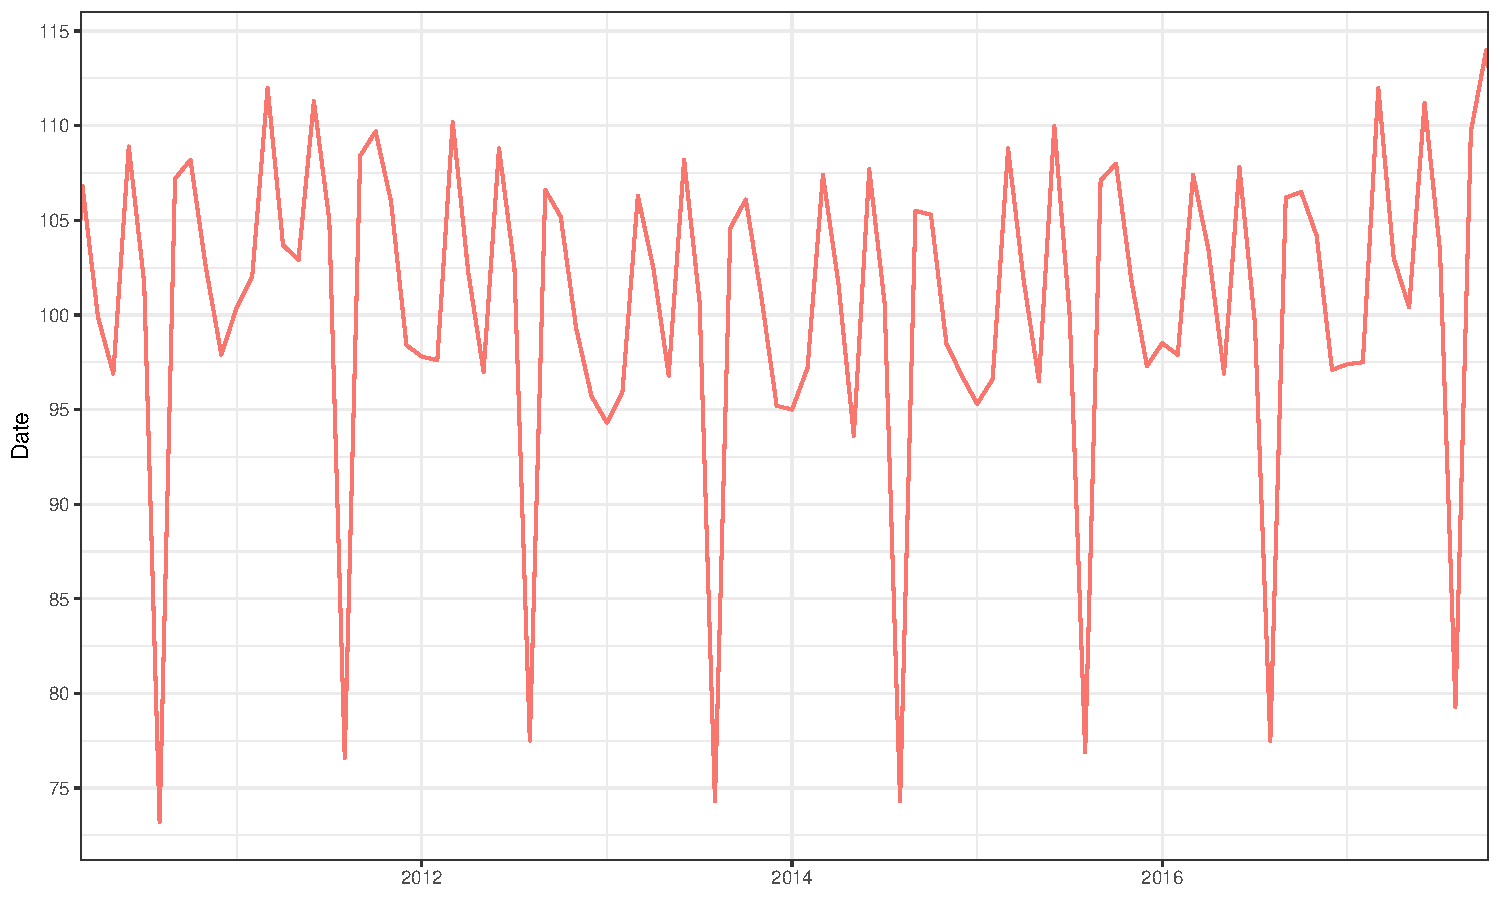
\includegraphics{img/markdown-unnamed-chunk-1-1.pdf}
\caption{Industrial production index in France}
\end{figure}

\end{frame}

\begin{frame}{Introduction to seasonal adjustment (2/3)}
\protect\hypertarget{introduction-to-seasonal-adjustment-23}{}

Purpose of seasonal adjustment:

\begin{itemize}
\tightlist
\item
  Time comparison (outlook, short-term evolution\ldots{})\\
\item
  Spatial comparison
\end{itemize}

\bigskip
\pause

Two leading methods:

\begin{itemize}
\tightlist
\item
  TRAMO/SEATS+ (Bank of Spain)\\
\item
  X-12ARIMA/X-13ARIMA-SEATS (US-Census Bureau).
\end{itemize}

\bigskip
\pause

\(\rightarrow\) proceed in two steps:

\begin{enumerate}
\item
  Pre-adjusting the series of deterministics effects with a RegARIMA
  model
\item
  Decomposition: to extract seasonal component
\end{enumerate}

\end{frame}

\begin{frame}{What's JDemetra+\bcquestion }
\protect\hypertarget{whats-jdemetra}{}


\includegraphics[width=2cm]{img/jdemetra+.png} TRAMO/SEATS+ and
X-13ARIMA-SEATS are implemented in JDemetra+ (JD+)

\bigskip

\large\faThumbsUp{} \normalsize Software
\href{https://ec.europa.eu/eurostat/cros/system/files/Jdemetra_\%20release.pdf}{officially
recommended} by Eurostat and the ECB for seasonal and calendar
adjustment of official statistics

\bigskip

\(\rightarrow\) RJDemetra is an \large\faRProject{}
\normalsize interface to JDemetra+ based on the \large\faJava{}
\normalsize libraries of JD+

\end{frame}

\hypertarget{rjdemetra}{%
\section{RJDemetra}\label{rjdemetra}}

\hypertarget{current-status}{%
\subsection{Current status}\label{current-status}}

\begin{frame}{Current status}
\protect\hypertarget{current-status-1}{}

\begin{itemize}
\tightlist
\item
  RegARIMA, TRAMO-SEATS and X-13-ARIMA:

  \begin{itemize}
  \tightlist
  \item
    pre-defined and user-defined specifications: outliers detection,
    ARIMA detection, userdefined regressors, transformation
    function\ldots{}\\
  \item
    S3 classes with plot, summary, print methods
  \end{itemize}
\end{itemize}

\medskip

\begin{itemize}
\tightlist
\item
  Manipulate JD+ workspaces:

  \begin{itemize}
  \tightlist
  \item
    Import JD+ workspace to get input raw series or SA model
  \item
    Export R models created via RJDemetra
  \end{itemize}
\end{itemize}

\medskip

\begin{itemize}
\tightlist
\item
  Include a dataset: industrial production indices in manufacturing in
  the European Union
\end{itemize}

\end{frame}

\begin{frame}[fragile]{Object structure}
\protect\hypertarget{object-structure}{}

A \texttt{SA} object is a \texttt{list()} of 5 elements:

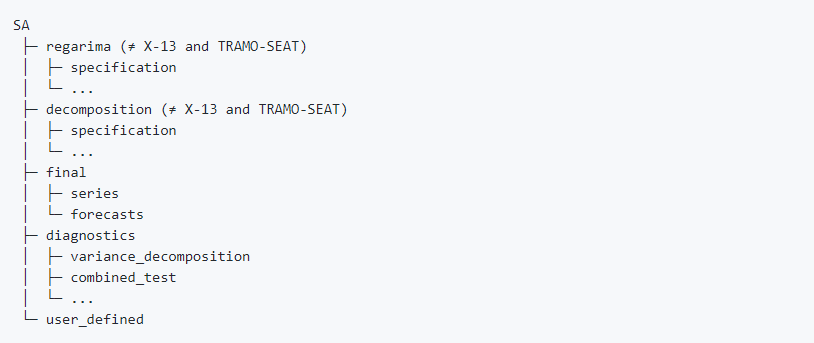
\includegraphics{img/sa_obj_struct.png}

\end{frame}

\begin{frame}[fragile]{Create your first model}
\protect\hypertarget{create-your-first-model}{}

Like in JD+ users can defined their own specification or use a
pre-defined one:

\footnotesize

\begin{Shaded}
\begin{Highlighting}[]
\KeywordTok{library}\NormalTok{(RJDemetra)}
\NormalTok{ipi_fr <-}\StringTok{ }\NormalTok{ipi_c_eu[, }\StringTok{"FR"}\NormalTok{]}
\NormalTok{ts_mod <-}\StringTok{ }\KeywordTok{tramoseats}\NormalTok{(ipi_fr, }\DataTypeTok{spec =} \StringTok{"RSAfull"}\NormalTok{)}
\NormalTok{x13_usr_spec <-}\StringTok{ }\KeywordTok{x13_spec}\NormalTok{(}\DataTypeTok{spec =} \KeywordTok{c}\NormalTok{(}\StringTok{"RSA5c"}\NormalTok{),}
                         \DataTypeTok{usrdef.outliersEnabled =} \OtherTok{TRUE}\NormalTok{,}
                         \DataTypeTok{usrdef.outliersType =} \KeywordTok{c}\NormalTok{(}\StringTok{"LS"}\NormalTok{, }\StringTok{"AO"}\NormalTok{),}
                         \DataTypeTok{usrdef.outliersDate =} \KeywordTok{c}\NormalTok{(}\StringTok{"2008-10-01"}\NormalTok{,}
                                                 \StringTok{"2002-01-01"}\NormalTok{),}
                         \DataTypeTok{usrdef.outliersCoef =} \KeywordTok{c}\NormalTok{(}\DecValTok{36}\NormalTok{, }\DecValTok{14}\NormalTok{),}
                         \DataTypeTok{transform.function =} \StringTok{"None"}\NormalTok{)}
\NormalTok{x13_mod <-}\StringTok{ }\KeywordTok{x13}\NormalTok{(ipi_fr, x13_usr_spec, }\DataTypeTok{userdefined =} \StringTok{"diagnostics.ic-ratio"}\NormalTok{)}
\end{Highlighting}
\end{Shaded}

Use \texttt{user\_defined\_variables()} to get the names of the
user-defined variables

\end{frame}

\hypertarget{regarima-examples}{%
\subsection{RegARIMA examples}\label{regarima-examples}}

\begin{frame}[fragile]{RegARIMA examples (1/2)}
\protect\hypertarget{regarima-examples-12}{}

\footnotesize

\begin{Shaded}
\begin{Highlighting}[]
\KeywordTok{summary}\NormalTok{(x13_mod}\OperatorTok{$}\NormalTok{regarima)}
\end{Highlighting}
\end{Shaded}

\begin{verbatim}
## y = regression model + arima (0, 1, 1, 0, 1, 1)
## 
## Model: RegARIMA - X13
## Estimation span: from 1-1990 to 12-2017
## Log-transformation: no
## Regression model: no mean, no trading days effect, no leap year effect, Easter effect, outliers(7)
## 
## Coefficients:
## ARIMA: 
##           Estimate Std. Error T-stat Pr(>|t|)    
## Theta(1)  -0.53675    0.04770 -11.25   <2e-16 ***
## BTheta(1) -0.50830    0.04961 -10.25   <2e-16 ***
## ---
## Signif. codes:  0 '***' 0.001 '**' 0.01 '*' 0.05 '.' 0.1 ' ' 1
## 
## Regression model: 
##              Estimate Std. Error  T-stat Pr(>|t|)    
## Easter [1]    -1.1686     0.3385  -3.452 0.000629 ***
## AO (9-2008)   31.4099     2.1812  14.400  < 2e-16 ***
## LS (9-2008)  -56.6477     2.2561 -25.109  < 2e-16 ***
## TC (9-2008)   24.1814     3.2563   7.426 1.00e-12 ***
## LS (2-2002)   14.7081     1.5257   9.640  < 2e-16 ***
## LS (12-2001) -14.6482     1.6811  -8.714  < 2e-16 ***
## AO (12-2001)  13.0297     1.7312   7.527 5.23e-13 ***
## LS (5-2008)   -5.4848     1.2957  -4.233 3.01e-05 ***
## ---
## Signif. codes:  0 '***' 0.001 '**' 0.01 '*' 0.05 '.' 0.1 ' ' 1
##              Coefficients
## LS (10-2008)           36
## AO (1-2002)            14
## 
## 
## Residual standard error: 1.729 on 11 degrees of freedom
## Log likelihood = -637.1, aic =  1296, aicc =  1297, bic(corrected for length) = 1.274
\end{verbatim}

\end{frame}

\begin{frame}[fragile]{RegARIMA examples (2/2)}
\protect\hypertarget{regarima-examples-22}{}

\begin{Shaded}
\begin{Highlighting}[]
\KeywordTok{layout}\NormalTok{(}\KeywordTok{matrix}\NormalTok{(}\DecValTok{1}\OperatorTok{:}\DecValTok{6}\NormalTok{, }\DecValTok{3}\NormalTok{, }\DecValTok{2}\NormalTok{));}\KeywordTok{plot}\NormalTok{(x13_mod}\OperatorTok{$}\NormalTok{regarima, }\DataTypeTok{ask =} \OtherTok{FALSE}\NormalTok{)}
\end{Highlighting}
\end{Shaded}

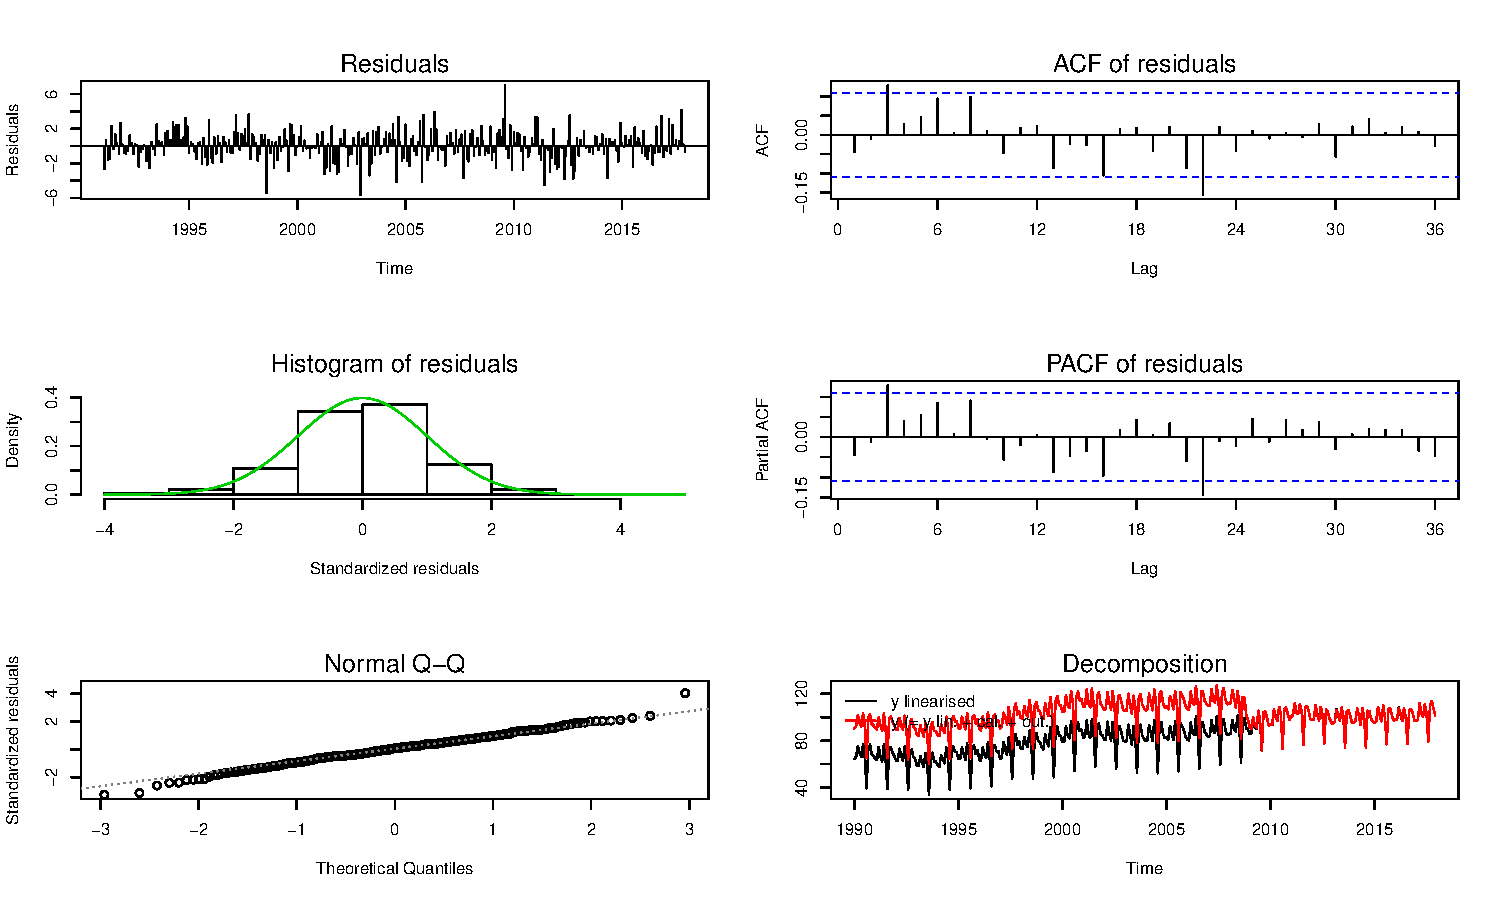
\includegraphics{img/markdown-unnamed-chunk-5-1.pdf}

\end{frame}

\hypertarget{seasonal-adjustment-examples}{%
\subsection{Seasonal adjustment
examples}\label{seasonal-adjustment-examples}}

\begin{frame}[fragile]{Seasonal adjustment examples (1/7):
decomposition}
\protect\hypertarget{seasonal-adjustment-examples-17-decomposition}{}

\footnotesize

\begin{Shaded}
\begin{Highlighting}[]
\NormalTok{x13_mod}\OperatorTok{$}\NormalTok{decomposition}
\end{Highlighting}
\end{Shaded}

\begin{verbatim}
##  Monitoring and Quality Assessment Statistics:  
##       M stats
## M(1)    0.055
## M(2)    0.041
## M(3)    0.926
## M(4)    0.621
## M(5)    0.724
## M(6)    0.215
## M(7)    0.074
## M(8)    0.208
## M(9)    0.056
## M(10)   0.158
## M(11)   0.146
## Q       0.297
## Q-M2    0.329
## 
## Final filters: 
## Seasonal filter:  3x5
## Trend filter:  13 terms Henderson moving average
\end{verbatim}

\end{frame}

\begin{frame}[fragile]{Seasonal adjustment examples (2/7):
decomposition}
\protect\hypertarget{seasonal-adjustment-examples-27-decomposition}{}

\footnotesize

\begin{Shaded}
\begin{Highlighting}[]
\NormalTok{ts_mod}\OperatorTok{$}\NormalTok{decomposition}
\end{Highlighting}
\end{Shaded}

\begin{verbatim}
## Model
## AR :  1 + 0.352498 B + 0.133616 B^2 
## D :  1 - B - B^12 + B^13 
## MA :  1 - 0.186819 B - 0.610856 B^12 + 0.114119 B^13 
## 
## 
## SA
## D :  1 - 2.000000 B + B^2 
## MA :  1 - 1.314459 B + 0.340427 B^2 
## Innovation variance:  0.4669153 
## 
## Trend
## D :  1 - 2.000000 B + B^2 
## MA :  1 + 0.040206 B - 0.959794 B^2 
## Innovation variance:  0.04869563 
## 
## Seasonal
## AR :  1 + 0.352498 B + 0.133616 B^2 
## D :  1 + B + B^2 + B^3 + B^4 + B^5 + B^6 + B^7 + B^8 + B^9 + B^10 + B^11 
## MA :  1 + 0.717848 B + 0.460721 B^2 + 0.310085 B^3 + 0.132447 B^4 - 0.049053 B^5 - 0.216655 B^6 - 0.354556 B^7 - 0.445030 B^8 - 0.469587 B^9 - 0.376625 B^10 - 0.166397 B^11 - 0.410618 B^12 - 0.132580 B^13 
## Innovation variance:  0.1601924 
## 
## Irregular
## Innovation variance:  0.2056884
\end{verbatim}

\end{frame}

\begin{frame}[fragile]{Seasonal adjustment examples (3/7)}
\protect\hypertarget{seasonal-adjustment-examples-37}{}

\begin{Shaded}
\begin{Highlighting}[]
\KeywordTok{plot}\NormalTok{(x13_mod}\OperatorTok{$}\NormalTok{decomposition)}
\end{Highlighting}
\end{Shaded}

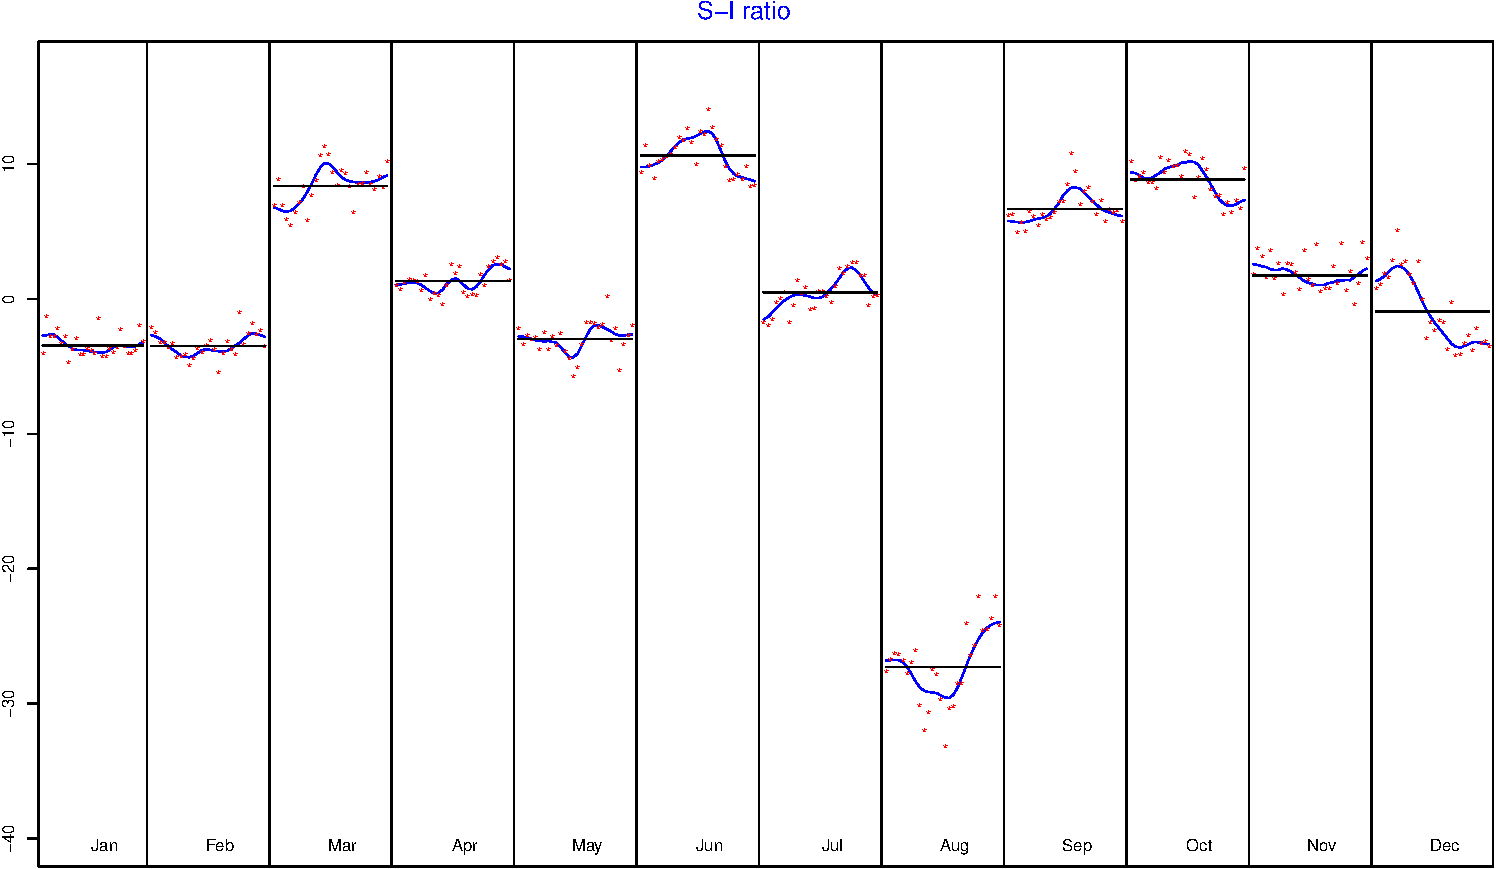
\includegraphics{img/markdown-unnamed-chunk-8-1.pdf}

\end{frame}

\begin{frame}[fragile]{Seasonal adjustment examples (4/7)}
\protect\hypertarget{seasonal-adjustment-examples-47}{}

\footnotesize

\begin{Shaded}
\begin{Highlighting}[]
\NormalTok{x13_mod}\OperatorTok{$}\NormalTok{final}
\end{Highlighting}
\end{Shaded}

\begin{verbatim}
## Last observed values
##              y       sa        t           s             i
## Jan 2017  97.4 100.6172 100.6174  -3.2172329 -0.0001992082
## Feb 2017  97.5 100.3127 101.0283  -2.8126932 -0.7155966863
## Mar 2017 112.0 102.5469 101.4894   9.4530696  1.0575376567
## Apr 2017 103.0 101.0897 101.9282   1.9103111 -0.8385432983
## May 2017 100.4 103.0319 102.3136  -2.6318733  0.7182480125
## Jun 2017 111.2 102.4926 102.6921   8.7074293 -0.1994894034
## Jul 2017 103.4 103.1596 103.0816   0.2404277  0.0779236963
## Aug 2017  79.3 103.2483 103.5055 -23.9483256 -0.2572170473
## Sep 2017 109.7 103.5536 103.9555   6.1464361 -0.4019376040
## Oct 2017 114.0 106.6886 104.3955   7.3113786  2.2931579296
## Nov 2017 107.7 105.4631 104.7505   2.2369236  0.7125546908
## Dec 2017 101.4 104.7490 105.0214  -3.3490189 -0.2723590878
## 
## Forecasts:
##                y_f     sa_f      t_f         s_f          i_f
## Jan 2018 101.96630 105.0963 105.1795  -3.1299775 -0.083200162
## Feb 2018 102.23632 105.1464 105.2838  -2.9100563 -0.137428535
## Mar 2018 113.85794 105.5026 105.3966   8.3553336  0.105971540
## Apr 2018 108.47477 105.4896 105.5573   2.9851827 -0.067754048
## May 2018 103.22164 105.7963 105.7844  -2.5746309  0.011859024
## Jun 2018 114.64042 106.0073 106.0629   8.6331483 -0.055612674
## Jul 2018 106.53519 106.3942 106.3666   0.1410119  0.027594337
## Aug 2018  82.77073 106.6890 106.6849 -23.9182264  0.004061745
## Sep 2018 112.79551 106.7018 106.9859   6.0936895 -0.284129714
## Oct 2018 115.13202 107.7516 107.2471   7.3803800  0.504589345
## Nov 2018 109.87965 107.5136 107.4572   2.3660966  0.056314698
## Dec 2018 103.97193 107.3744 107.6093  -3.4024325 -0.234923742
\end{verbatim}

\end{frame}

\begin{frame}[fragile]{Seasonal adjustment examples (5/7)}
\protect\hypertarget{seasonal-adjustment-examples-57}{}

\begin{Shaded}
\begin{Highlighting}[]
\KeywordTok{plot}\NormalTok{(x13_mod}\OperatorTok{$}\NormalTok{final, }\DataTypeTok{first_date =} \DecValTok{2012}\NormalTok{, }\DataTypeTok{type_chart =} \StringTok{"sa-trend"}\NormalTok{)}
\end{Highlighting}
\end{Shaded}

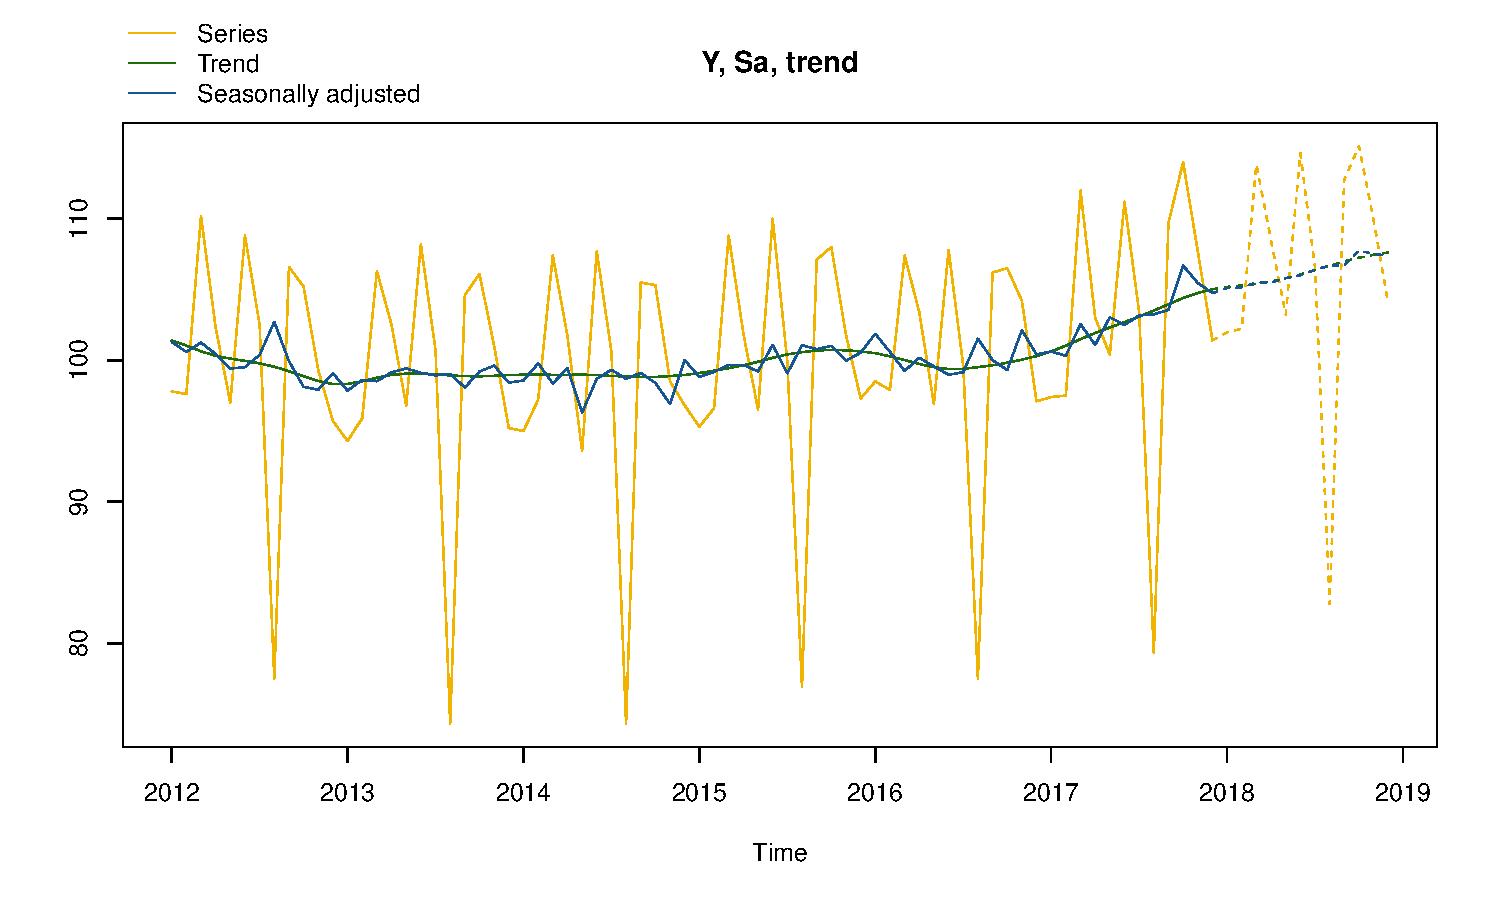
\includegraphics{img/markdown-unnamed-chunk-10-1.pdf}

\end{frame}

\begin{frame}[fragile]{Seasonal adjustment examples (6/7)}
\protect\hypertarget{seasonal-adjustment-examples-67}{}

\begin{Shaded}
\begin{Highlighting}[]
\KeywordTok{plot}\NormalTok{(x13_mod}\OperatorTok{$}\NormalTok{final, }\DataTypeTok{last_date =} \DecValTok{2000}\NormalTok{, }\DataTypeTok{type_chart =} \StringTok{"cal-seas-irr"}\NormalTok{)}
\end{Highlighting}
\end{Shaded}

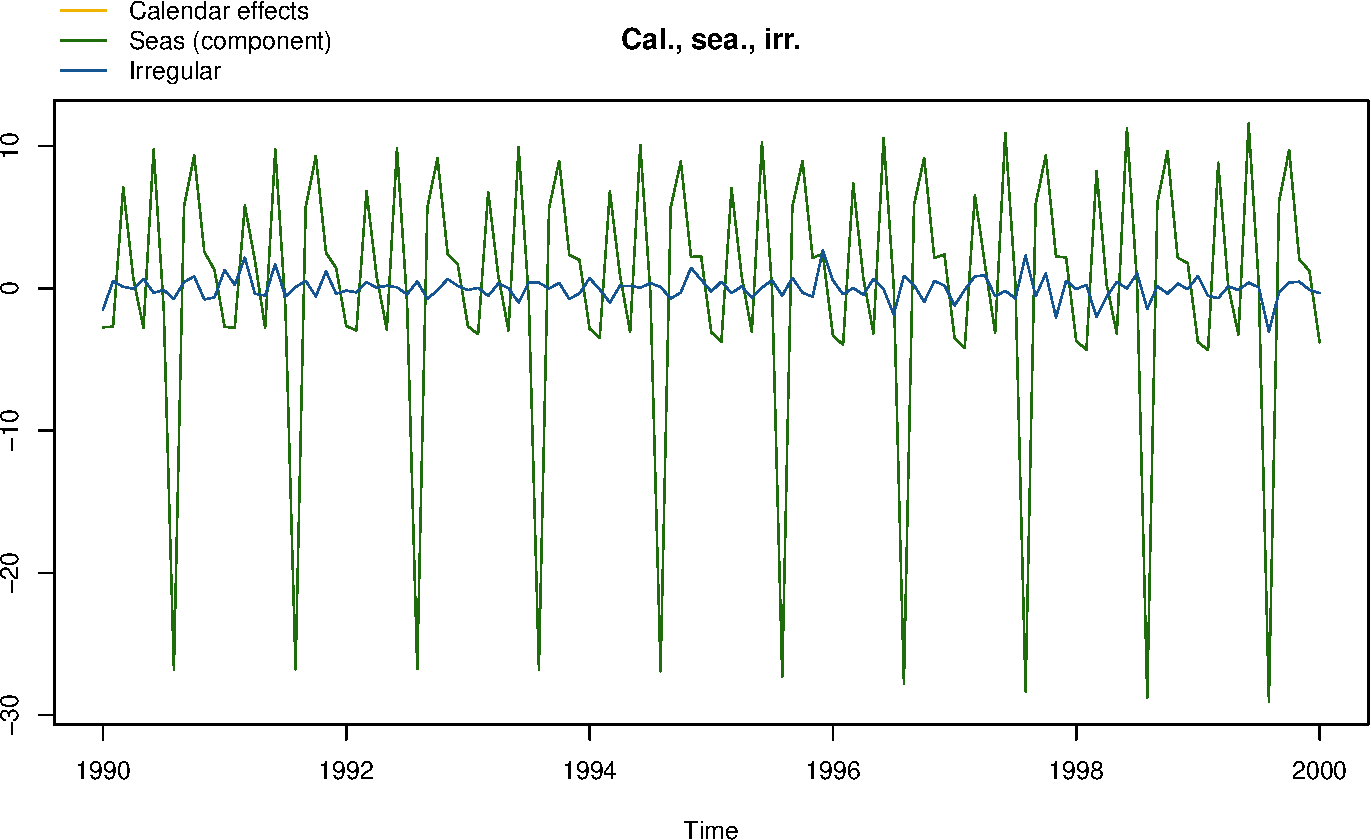
\includegraphics{img/markdown-unnamed-chunk-11-1.pdf}

\end{frame}

\begin{frame}[fragile]{Seasonal adjustment examples (7/7)}
\protect\hypertarget{seasonal-adjustment-examples-77}{}

\footnotesize

\begin{Shaded}
\begin{Highlighting}[]
\NormalTok{x13_mod}\OperatorTok{$}\NormalTok{diagnostics}
\end{Highlighting}
\end{Shaded}

\begin{verbatim}
##  Relative contribution of the components to the stationary
##  portion of the variance in the original series,
##  after the removal of the long term trend 
##  Trend computed by Hodrick-Prescott filter (cycle length = 8.0 years)
##            Component
##  Cycle         1.557
##  Seasonal     39.219
##  Irregular     0.362
##  TD & Hol.     0.018
##  Others       61.971
##  Total       103.128
## 
##  Combined test in the entire series 
##  Non parametric tests for stable seasonality
##                                                           P.value
##    Kruskall-Wallis test                                      0.000
##    Test for the presence of seasonality assuming stability   0.000
##    Evolutive seasonality test                                0.032
##  
##  Identifiable seasonality present
## 
##  Residual seasonality tests 
##                                       P.value
##  qs test on sa                          1.000
##  qs test on i                           1.000
##  f-test on sa (seasonal dummies)        0.997
##  f-test on i (seasonal dummies)         0.965
##  Residual seasonality (entire series)   0.993
##  Residual seasonality (last 3 years)    0.922
##  f-test on sa (td)                      0.001
##  f-test on i (td)                       0.006
\end{verbatim}

\end{frame}

\hypertarget{export-a-jd-workspace}{%
\subsection{Export a JD+ workspace}\label{export-a-jd-workspace}}

\begin{frame}[fragile]{Export a workspace}
\protect\hypertarget{export-a-workspace}{}

\footnotesize

\begin{Shaded}
\begin{Highlighting}[]
\NormalTok{wk <-}\StringTok{ }\KeywordTok{new_workspace}\NormalTok{()}
\KeywordTok{new_multiprocessing}\NormalTok{(wk, }\DataTypeTok{name =} \StringTok{"MP-1"}\NormalTok{)}
\KeywordTok{add_sa_item}\NormalTok{(wk, }\DataTypeTok{multiprocessing =} \StringTok{"MP-1"}\NormalTok{,}
            \DataTypeTok{sa_obj =}\NormalTok{ x13_mod, }\DataTypeTok{name =}  \StringTok{"SA with X13 model 1 "}\NormalTok{)}
\KeywordTok{add_sa_item}\NormalTok{(wk, }\DataTypeTok{multiprocessing =}  \StringTok{"MP-1"}\NormalTok{,}
            \DataTypeTok{sa_obj =}\NormalTok{ ts_mod, }\DataTypeTok{name =} \StringTok{"SA with TramoSeats model 1"}\NormalTok{)}
\KeywordTok{save_workspace}\NormalTok{(wk, }\StringTok{"workspace.xml"}\NormalTok{)}
\end{Highlighting}
\end{Shaded}

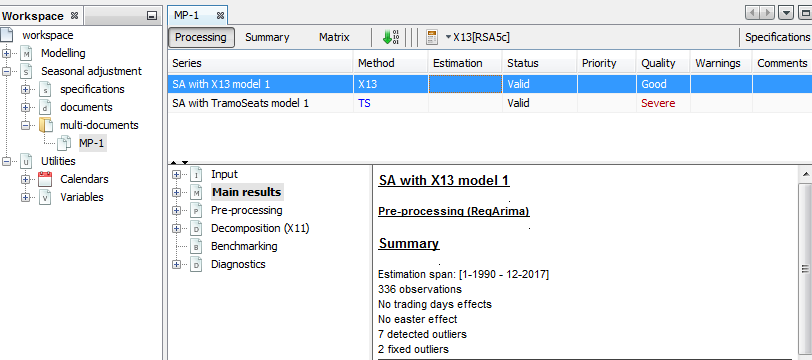
\includegraphics{img/workspace.png}

\end{frame}

\hypertarget{import-a-jd-workspace}{%
\subsection{Import a JD+ workspace}\label{import-a-jd-workspace}}

\begin{frame}[fragile]{Import a workspace}
\protect\hypertarget{import-a-workspace}{}

\footnotesize

\begin{Shaded}
\begin{Highlighting}[]
\NormalTok{wk <-}\StringTok{ }\KeywordTok{load_workspace}\NormalTok{(}\StringTok{"workspace.xml"}\NormalTok{)}
\KeywordTok{compute}\NormalTok{(wk) }\CommentTok{# Important to get the Sa model}
\NormalTok{models <-}\StringTok{ }\KeywordTok{get_model}\NormalTok{(wk, }\DataTypeTok{progress_bar =} \OtherTok{FALSE}\NormalTok{) }\CommentTok{# get all models}
\CommentTok{# Or to get one specific model:}
\NormalTok{mp <-}\StringTok{ }\KeywordTok{get_object}\NormalTok{(wk, }\DecValTok{1}\NormalTok{)}
\KeywordTok{count}\NormalTok{(mp)}
\end{Highlighting}
\end{Shaded}

\begin{verbatim}
## [1] 2
\end{verbatim}

\begin{Shaded}
\begin{Highlighting}[]
\NormalTok{sa2 <-}\StringTok{ }\KeywordTok{get_object}\NormalTok{(mp, }\DecValTok{2}\NormalTok{)}
\KeywordTok{get_name}\NormalTok{(sa2)}
\end{Highlighting}
\end{Shaded}

\begin{verbatim}
## [1] "SA with TramoSeats model 1"
\end{verbatim}

\begin{Shaded}
\begin{Highlighting}[]
\NormalTok{mod <-}\StringTok{ }\KeywordTok{get_model}\NormalTok{(sa2, wk)}
\end{Highlighting}
\end{Shaded}

\end{frame}

\hypertarget{reduce-time-computation}{%
\subsection{Reduce time computation}\label{reduce-time-computation}}

\begin{frame}[fragile]{Manipulate \faJava{} objects (1/2)}
\protect\hypertarget{manipulate-objects-12}{}

\footnotesize

Default functions can be time consuming (computation of outputs)\ldots{}
Especially if you only need one specific parameter

\(\rightarrow\) ``Manipulate'' java models: \texttt{jx13},
\texttt{jtramoseats}, \texttt{jregarima}, \texttt{jregarima\_x13},
\texttt{jregarima\_tramoseats} and \texttt{get\_jmodel}

\begin{Shaded}
\begin{Highlighting}[]
\NormalTok{jx13_mod <-}\StringTok{ }\KeywordTok{jx13}\NormalTok{(ipi_fr, x13_usr_spec)}
\CommentTok{# To get the available outputs:}
\KeywordTok{tail}\NormalTok{(}\KeywordTok{get_dictionary}\NormalTok{(jx13_mod), }\DecValTok{2}\NormalTok{)}
\end{Highlighting}
\end{Shaded}

\begin{verbatim}
## [1] "diagnostics.msr-global" "diagnostics.msr(*)"
\end{verbatim}

\begin{Shaded}
\begin{Highlighting}[]
\CommentTok{# To get an indicator:}
\KeywordTok{get_indicators}\NormalTok{(jx13_mod, }\StringTok{"diagnostics.td-res-all"}\NormalTok{, }\StringTok{"diagnostics.ic-ratio"}\NormalTok{)}
\end{Highlighting}
\end{Shaded}

\begin{verbatim}
## $`diagnostics.td-res-all`
## [1] 3.020374254 0.006933563
## attr(,"description")
## [1] "F with 6 degrees of freedom in the nominator and 317 degrees of freedom in the denominator"
## 
## $`diagnostics.ic-ratio`
## [1] 4.356533
\end{verbatim}

\begin{Shaded}
\begin{Highlighting}[]
\CommentTok{# To get the previous R output}
\NormalTok{x13_mod <-}\StringTok{ }\KeywordTok{jSA2R}\NormalTok{(jx13_mod)}
\end{Highlighting}
\end{Shaded}

\(\rightarrow\) The output can be customize by every user/institute

\end{frame}

\hypertarget{around-rjdemetra-and-jdemetra}{%
\section{Around RJDemetra and
JDemetra+}\label{around-rjdemetra-and-jdemetra}}

\hypertarget{around-rjdemetra}{%
\subsection{Around RJDemetra}\label{around-rjdemetra}}

\begin{frame}{Examples of current use of RJDemetra}
\protect\hypertarget{examples-of-current-use-of-rjdemetra}{}

\begin{itemize}
\tightlist
\item
  ggdemetra: ggplot2 extension for `RJDemetra'
\end{itemize}

\faGithub{} \url{https://github.com/AQLT/rjdqa}

\begin{itemize}
\tightlist
\item
  rjdqa: package to help quality assessment (dashboard and quality
  report matrix)
\end{itemize}

\faGithub{} \url{https://github.com/AQLT/rjdqa}

\begin{itemize}
\tightlist
\item
  persephone: enable easy processing during production of SA series
  (interactive plots, dashboards\ldots{})
\end{itemize}

\faGithub{} \url{https://github.com/statistikat/persephone}

\begin{itemize}
\tightlist
\item
  rjdmarkown: nice rmarkdown outputs for RJDemetra
\end{itemize}

\faGithub{} \url{https://github.com/AQLT/rjdmarkdown}

\begin{itemize}
\tightlist
\item
  Carry out studies on SA: Ladiray D., Quartier-la-Tente A.,
  ``(In)Stability of Reg-ARIMA Models for Seasonal Adjustment''
\end{itemize}

\end{frame}

\hypertarget{around-jdemetra}{%
\subsection{Around JDemetra+}\label{around-jdemetra}}

\begin{frame}{Around JDemetra+}
\protect\hypertarget{around-jdemetra-1}{}

\begin{itemize}
\tightlist
\item
  State space framework of JD+:\\
  \faGithub{} \url{https://github.com/nbbrd/rjdssf}
\end{itemize}

\medskip

\begin{itemize}
\tightlist
\item
  Benchmarking and temporal disaggregation:\\
  \faGithub{} \url{https://github.com/palatej/rjdbench}
\end{itemize}

\medskip

\begin{itemize}
\tightlist
\item
  R interface to the JWSACruncher (console tool to refresh the models of
  a JD+ workspace:\\
  \faGithub{} \url{https://github.com/AQLT/rjwsacruncher}
\end{itemize}

\end{frame}

\hypertarget{installation-and-future-developments}{%
\section{Installation and future
developments}\label{installation-and-future-developments}}

\hypertarget{how-to-install-the-package}{%
\subsection{How to install the
package?}\label{how-to-install-the-package}}

\begin{frame}[fragile]{How to install the package?}
\protect\hypertarget{how-to-install-the-package-1}{}

The package is available on \large\faGithub\normalsize:
\url{https://github.com/jdemetra/rjdemetra}

It has also it's own website:
\url{https://jdemetra.github.io/rjdemetra/}

\begin{Shaded}
\begin{Highlighting}[]
\CommentTok{# Cran release}
\KeywordTok{install.packages}\NormalTok{(}\StringTok{"RJDemetra"}\NormalTok{)}

\CommentTok{# Development version}
\NormalTok{devtools}\OperatorTok{::}\KeywordTok{install_github}\NormalTok{(}\StringTok{"jdemetra/rjdemetra"}\NormalTok{)}
\end{Highlighting}
\end{Shaded}

\bcinfo To install it you need Java8: in case you don't, install a
portable version of Java8 and set the \texttt{JAVA\_HOME} path.

See the installation manual:
\url{https://github.com/jdemetra/rjdemetra/wiki/Installation-manual}

\end{frame}

\begin{frame}[fragile]{Why use RJDemetra \bcquestion}
\protect\hypertarget{why-use-rjdemetra}{}

\begin{itemize}
\item
  Methods used are recommended by Eurostat
\item
  Performance and integration in production with JDemetra+
\item
  Lots of \large\faRProject{} \normalsize developments around
  \texttt{RJDemetra}
\item
  \texttt{RJDemetra} evolves with JDemetra+: will integrate new
  developments on SA methods
\end{itemize}

\end{frame}

\hypertarget{future-developments}{%
\subsection{Future developments}\label{future-developments}}

\begin{frame}{What's next? \bcpanchant}
\protect\hypertarget{whats-next}{}

\begin{itemize}
\item
  documentation: article for the Journal of Statistical Software + cheat
  sheet
\item
  shiny app to change the specification
\end{itemize}

With JD+ 3.0.0 (by the end of 2020):

\begin{itemize}
\item
  Function to ``refresh'' the model
\item
  Compatibility with all frequencies (JD+ daily, weekly, etc.)
\end{itemize}

\end{frame}

\begin{frame}{Thank you for your attention\ldots{}}
\protect\hypertarget{thank-you-for-your-attention}{}

\ldots{} And don't forget your stickers!

\medskip

\begin{columns}
\begin{column}{0.33\textwidth}
\begin{center}

\includegraphics[width=\textwidth]{img/rjdemetra_logo.png}
\end{center}
\end{column}
\begin{column}{0.33\textwidth}
\begin{center}

\includegraphics[width=3cm]{img/jdemetra+.png}
\end{center}
\end{column}
\begin{column}{0.33\textwidth} 
\begin{center}

\includegraphics[width=3cm]{img/ggdemetra_logo.png}
\end{center}
\end{column}
\end{columns}

\bigskip
\bigskip

\begin{columns}
\begin{column}{0.5\textwidth}
Alain Quartier-la-Tente


\href{mailto:alain.quartier-la-tente@insee.fr}{\faEnvelope{} alain.quartier-la-tente@insee.fr} 
\end{column}
\begin{column}{0.5\textwidth} 
\href{https://github.com/jdemetra/rjdemetra}{\faGithub{} jdemetra/rjdemetra}  

\href{https://twitter.com/JDemetraPlus}{\faTwitter{} @JdemetraPlus}

\end{column}
\end{columns}

\end{frame}

\end{document}
